\documentclass[11pt,twoside,openright]{book}

% =============================================================================
% Mass Spectrometry Data Analysis with R
% Chapter 20: Experimental Design, Replication, and Power in Mass Spectrometry
% Author: Lucas VHH TRAN (CK-CARE Davos)
% Style: Springer Nature Monograph (Health Analytics with R Pedagogy)
% =============================================================================

\usepackage{springer_monograph}
\usepackage{placeins}
\usepackage{float}

\hypersetup{
    pdftitle={Chapter 20: Experimental Design, Replication, and Power in Mass Spectrometry},
    pdfauthor={Lucas VHH TRAN}
}

\begin{document}

% --- Chapter Title Block ---
\setcounter{chapter}{19}
\chapter{Experimental Design, Replication, and Power in Mass Spectrometry}
\label{ch:experimental_design}

\noindent
\textbf{Lucas VHH TRAN}\footnote{CK-CARE Davos, Christine K\"uhne -- Center for Allergy Research and Education, Davos, Switzerland. Email: \texttt{lucas.tran@ck-care.ch}}\\
\rule{\textwidth}{0.8pt}

\begin{abstract}
\noindent
Mass spectrometers suffer from time-dependent signal drift, electrospray source fouling, chromatographic retention time shifts, and batch-to-batch variation. No downstream statistical algorithm or normalization formula can rescue a study when biological conditions are confounded with technical acquisition batches. This chapter establishes the mathematical principles, physical error structures, and computational tools required to design valid mass spectrometry studies. We formulate the Fisherian triad---replication, randomization, and local control (blocking) \cite{fisher1935design, box1978statistics}---within the context of high-dimensional chromatography and mass spectrometry \cite{graw2020statistical, broadhurst2018guidelines}. We decompose experimental variance into biological and technical components, derive the intraclass correlation coefficient \cite{shrout1979intraclass}, and demonstrate the diminishing returns of repeated technical injections \cite{hurlbert1984pseudoreplication}. We provide exact analytical power formulations under multiple testing adjustments (Benjamini--Hochberg false discovery rate control \cite{benjamini1995controlling, cohen1988statistical}) and left-censored feature dropout \cite{karpievitch2012normalization, hoenig2001abuse}. Through an executable R laboratory, we implement randomized complete block designs \cite{fisher1935design, box1978statistics}, pre-acquisition confounding diagnostic audits \cite{leek2010tackling, johnson2007adjusting}, empirical Bayes power simulations with \texttt{limma} \cite{smyth2004linear, ritchie2015limma, choi2014msstats}, and duplicate correlation modeling to prevent pseudoreplication \cite{hurlbert1984pseudoreplication, kammers2015detecting, vanderaa2021scp}. The chapter concludes with the Five Deadly Sins of mass spectrometry experimental design, a self-assessment checklist, and four multi-tier exercises with complete worked solutions.
\end{abstract}

\noindent
\textbf{Keywords:}\enspace Experimental Design, Randomized Complete Block Design (RCBD), Pseudoreplication, Intraclass Correlation Coefficient (ICC), Statistical Power, False Discovery Rate (FDR), Batch Confounding, limma, Quality Control.

\vspace{0.8em}
\noindent\rule{\textwidth}{0.4pt}

% =============================================================================
% Methodological Roadmap
% =============================================================================

\begin{table}[ht]
\centering
\caption{Methodological Roadmap: Four Stages of Experimental Design in Mass Spectrometry}
\label{tab:design_roadmap}
\small
\begin{tabularx}{\textwidth}{l p{3.8cm} p{4.2cm} X}
\toprule
\textbf{Stage} & \textbf{Physical Mechanism} & \textbf{Key Analytical Objective} & \textbf{Primary Failure Mode \& Remedy} \\
\midrule
\textbf{1. Replicate Allocation} & Biological diversity vs instrument measurement error; ICC $= \sigma^2_{\text{bio}} / (\sigma^2_{\text{bio}} + \sigma^2_{\text{tech}})$ \cite{shrout1979intraclass, hurlbert1984pseudoreplication}. & Allocate resources between biological units ($n$) and technical injections ($m$). & Pseudoreplication: treating $m$ injections as independent $N = n \cdot m$. Remedy: Average injections or apply \texttt{duplicateCorrelation()} \cite{smyth2004linear}. \\
\addlinespace
\textbf{2. Blocking Architecture} & Multi-well plates, digestion batches, TMT plexes, and instrument days \cite{fisher1935design, box1978statistics}. & Balance biological groups evenly across technical blocks (RCBD). & Complete confounding: all cases in Batch 1, all controls in Batch 2. Remedy: Orthogonal randomized complete block design \cite{leek2010tackling, johnson2007adjusting}. \\
\addlinespace
\textbf{3. Sequence Randomization} & Source contamination, column aging, mass calibration drift, and carryover \cite{broadhurst2018guidelines, graw2020statistical}. & Break correlation between injection order and biological condition. & Monotonic drift mistaken for biological induction. Remedy: Constrained run randomization with periodic pooled QCs. \\
\addlinespace
\textbf{4. Power Planning} & Multiplicity ($M = 10^3$--$10^4$ tests) and left-censored dropout ($p_{\text{miss}}$) \cite{karpievitch2012normalization, hoenig2001abuse}. & Calculate required $n$ under target FDR ($q \le 0.05$) and missingness. & Underpowered studies ($n=3$ for human plasma). Remedy: FDR-inflated and missingness-adjusted sample size formulas \cite{benjamini1995controlling, cohen1988statistical}. \\
\bottomrule
\end{tabularx}
\end{table}

\FloatBarrier

\begin{notebox}
\textbf{Tutor's Methodological Advice: The Orthogonality Principle}\\
Never allow a biological variable of interest to align with a technical unit of processing. If every diseased tissue is digested on Monday and every healthy control on Tuesday, the treatment effect is mathematically unidentifiable from the day effect. No statistical method, whether \texttt{ComBat}, linear mixed models, or deep learning, can separate biology from batch when the design matrix is collinear. Balance every plate, every digestion day, and every isobaric multiplex across conditions before collecting data.
\end{notebox}

% =============================================================================
\section{Biophysical and Mathematical Foundations}
% =============================================================================

\subsection{The Fisherian Triad in Liquid Chromatography--Mass Spectrometry}

Ronald A. Fisher established three foundational requirements for experimental validity: replication, randomization, and local control (blocking) \cite{fisher1935design}. In liquid chromatography coupled to mass spectrometry (LC-MS), these principles map directly to physical sources of analytical variance:

\begin{enumerate}
    \item \textbf{Replication}: Distinguishes biological variability from analytical error. Biological replicates represent independent organisms, patients, or cell culture passages. Technical replicates represent repeated preparation or repeated instrumental injections of the same biological material.
    \item \textbf{Randomization}: Converts deterministic instrument drift into independent, identically distributed noise. Mass spectrometers undergo non-stationary degradation: electrospray ionization (ESI) emitters accumulate non-volatile salts, quadrupole transmission curves drift with temperature, and reversed-phase columns lose resolving power over hundreds of injections \cite{broadhurst2018guidelines, graw2020statistical}. Randomizing the injection sequence ensures that time-dependent drift does not correlate with biological groups.
    \item \textbf{Local Control (Blocking)}: Partitions known sources of technical heterogeneity into homogeneous sub-units. Typical blocks include 96-well extraction plates, tryptic digestion rounds, instrument calibration intervals, and isobaric labeling plexes (TMT or iTRAQ). Balancing conditions within each block allows the removal of block-to-block variance without losing degrees of freedom for the biological contrast \cite{box1978statistics}.
\end{enumerate}

\subsection{Hierarchical Variance Decomposition and the Intraclass Correlation}

Consider the quantitative readout $y_{ijk}$ (on the $\log_2$ intensity scale) for feature $g$ in biological subject $j$ of condition $i$ during technical injection $k$:
\begin{equation}
y_{ijk} = \mu + \alpha_i + b_{ij} + e_{ijk}
\label{eq:hierarchical_model}
\end{equation}
where $\mu$ is the baseline mean, $\alpha_i$ is the fixed biological effect of condition $i$ with $\sum_i \alpha_i = 0$, $b_{ij} \sim \mathcal{N}(0, \sigma^2_{\text{bio}})$ is the random biological effect of subject $j$, and $e_{ijk} \sim \mathcal{N}(0, \sigma^2_{\text{tech}})$ is the random technical error.

For a group mean $\bar{y}_{i\cdot\cdot}$ estimated from $n$ biological subjects, each measured with $m$ technical injections, the total variance is:
\begin{equation}
\operatorname{Var}(\bar{y}_{i\cdot\cdot}) = \frac{\sigma^2_{\text{bio}}}{n} + \frac{\sigma^2_{\text{tech}}}{n \cdot m}
\label{eq:var_mean}
\end{equation}

The proportion of total variance attributable to genuine biological variation is the \textbf{Intraclass Correlation Coefficient (ICC)}:
\begin{equation}
\text{ICC} = \rho = \frac{\sigma^2_{\text{bio}}}{\sigma^2_{\text{bio}} + \sigma^2_{\text{tech}}}
\label{eq:icc}
\end{equation}

\vspace{0.6em}
\noindent\textbf{Theorem 20.1 (Diminishing Returns of Technical Replication).}\enspace
\textit{Let the total variance of the estimated treatment mean be defined as in Eq.~\eqref{eq:var_mean}. As the number of technical injections per subject $m \to \infty$, the variance asymptotically approaches a non-zero lower bound governed strictly by biological replication:
\begin{equation}
\lim_{m \to \infty} \operatorname{Var}(\bar{y}_{i\cdot\cdot}) = \frac{\sigma^2_{\text{bio}}}{n}
\end{equation}
Consequently, when biological variance exceeds technical variance ($\text{ICC} > 0.50$), increasing biological sample size $n$ reduces total variance faster than increasing technical replicates $m$.}

\vspace{0.6em}
\noindent\textbf{Proof.}\enspace
Differentiating Eq.~\eqref{eq:var_mean} with respect to $n$ and $m$ yields the marginal variance reductions:
\begin{align}
\frac{\partial \operatorname{Var}}{\partial n} &= -\frac{\sigma^2_{\text{bio}}}{n^2} - \frac{\sigma^2_{\text{tech}}}{n^2 m} = -\frac{1}{n} \operatorname{Var}(\bar{y}_{i\cdot\cdot}) \\
\frac{\partial \operatorname{Var}}{\partial m} &= -\frac{\sigma^2_{\text{tech}}}{n m^2}
\end{align}
The ratio of marginal gains is:
\begin{equation}
\frac{|\partial \operatorname{Var} / \partial n|}{|\partial \operatorname{Var} / \partial m|} = \frac{m \sigma^2_{\text{bio}} + \sigma^2_{\text{tech}}}{\sigma^2_{\text{tech}} / m} = m \left( 1 + m \frac{\sigma^2_{\text{bio}}}{\sigma^2_{\text{tech}}} \right)
\end{equation}
When $\sigma^2_{\text{bio}} \gg \sigma^2_{\text{tech}}$ (e.g., in human clinical cohorts where ICC $\ge 0.85$), the ratio exceeds $m(1 + 5.67m) > 1$. Adding an extra biological replicate provides greater reduction in estimation variance than adding repeated technical injections. \hfill $\blacksquare$
\vspace{0.6em}

\subsection{Cost-Constrained Optimal Allocation}

When resources are constrained by sample preparation costs $c_{\text{bio}}$ and instrument acquisition costs $c_{\text{tech}}$, the total cost per experimental group is:
\begin{equation}
C = n \cdot c_{\text{bio}} + n \cdot m \cdot c_{\text{tech}} = n (c_{\text{bio}} + m \cdot c_{\text{tech}})
\label{eq:cost_constraint}
\end{equation}

Minimizing $\operatorname{Var}(\bar{y}_{i\cdot\cdot}) = \frac{\sigma^2_{\text{bio}}}{n} + \frac{\sigma^2_{\text{tech}}}{n m}$ subject to budget $C$ using Lagrange multipliers yields the optimal technical replicate count $m^*$:
\begin{equation}
m^* = \frac{\sigma_{\text{tech}}}{\sigma_{\text{bio}}} \sqrt{\frac{c_{\text{bio}}}{c_{\text{tech}}}}
\label{eq:optimal_m}
\end{equation}
In standard untargeted proteomics, sample preparation is often less costly than instrument run time ($c_{\text{bio}} < c_{\text{tech}}$), and $\sigma_{\text{bio}} > \sigma_{\text{tech}}$. In such settings, $m^* < 1$, which confirms that a single injection per biological replicate ($m = 1$) is mathematically optimal. Multiple technical injections become justified only when sample collection is exceptionally expensive or when technical error exceeds biological variation, as observed in single-cell proteomics \cite{vanderaa2021scp}.

\subsection{Analytical Power and Sample Size Under Multiplicity}

Statistical power ($1 - \beta$) is the probability of rejecting the null hypothesis $H_0: \mu_1 = \mu_2$ when a true difference of magnitude $\delta$ exists. For a two-sample two-sided $t$-test with equal group sizes $n$, the test statistic follows a non-central $t$-distribution:
\begin{equation}
T = \frac{\bar{y}_1 - \bar{y}_2}{s_p \sqrt{2/n}} \sim t_{2n-2}(\theta), \quad \theta = \frac{\delta}{\sigma \sqrt{2/n}} = \frac{d \sqrt{n}}{\sqrt{2}}
\label{eq:nct}
\end{equation}
where $d = \delta / \sigma$ is Cohen's standardized effect size and $s_p$ is the pooled sample standard deviation.

Under a Gaussian approximation, the required sample size per group at significance level $\alpha$ and power $1 - \beta$ is:
\begin{equation}
n = \frac{2 \left( z_{1 - \alpha/2} + z_{1 - \beta} \right)^2 \sigma^2}{\delta^2} = \frac{2 \left( z_{1 - \alpha/2} + z_{1 - \beta} \right)^2}{d^2}
\label{eq:analytical_n}
\end{equation}
where $z_p$ is the $p$-th quantile of the standard normal distribution.

In untargeted omics, testing $M$ features simultaneously ($M = 3,000$ to $10,000$) requires controlling the false discovery rate (FDR) \cite{benjamini1995controlling}. Under the conservative Bonferroni threshold for family-wise error rate (FWER) or target FDR $q$:
\begin{equation}
\alpha^* = \frac{q}{M}
\label{eq:bonferroni_alpha}
\end{equation}
For $M = 5,000$ and $q = 0.05$, the per-test critical threshold drops to $\alpha^* = 1.0 \times 10^{-5}$. This shifts the critical normal quantile $z_{1 - \alpha^*/2}$ from $1.960$ to $4.417$. The required sample size increases by a factor of approximately:
\begin{equation}
\text{Inflation Factor} = \left( \frac{z_{1 - \alpha^*/2} + z_{1 - \beta}}{z_{1 - \alpha/2} + z_{1 - \beta}} \right)^2 = \left( \frac{4.417 + 0.842}{1.960 + 0.842} \right)^2 = \left( \frac{5.259}{2.802} \right)^2 \approx 3.52
\end{equation}
A study requiring $n = 9$ subjects for a single test requires at least $n = 32$ subjects per group when evaluating 5,000 features simultaneously.

\subsection{Inflation for Left-Censored Missing Values}

Mass spectrometry data contains non-random missingness caused by low precursor ionization, ion suppression, and detection limits (Chapter 19) \cite{karpievitch2012normalization}. If a feature has missingness proportion $p_{\text{miss}}$, the effective sample size available for testing is reduced:
\begin{equation}
n_{\text{eff}} = n \cdot (1 - p_{\text{miss}})
\label{eq:n_effective}
\end{equation}
To preserve nominal statistical power ($n_{\text{req}}$) for features subject to analytical dropout, the enrolled cohort size $n^*$ must be inflated:
\begin{equation}
n^* = \left\lceil \frac{n_{\text{req}}}{1 - p_{\text{miss}}} \right\rceil
\label{eq:n_inflated}
\end{equation}
When $n_{\text{req}} = 32$ and expected dropout is $p_{\text{miss}} = 0.25$, the study must enroll $n^* = \lceil 32 / 0.75 \rceil = 43$ subjects per group.

% =============================================================================
\section{Algorithmic Architecture and Study Designs}
% =============================================================================

\subsection{Randomized Complete Block Designs (RCBD)}

When samples exceed the capacity of a single processing unit (e.g., a 96-well digestion plate or an isobaric labeling batch), samples must be partitioned into blocks. An unblocked allocation risks placing all diseased samples on one plate and all healthy controls on another, rendering the treatment effect collinear with plate effects.

In a Randomized Complete Block Design (RCBD), each block contains an equal number of samples from every biological condition:
\begin{equation}
n_{ij} = \frac{n_i}{B}
\end{equation}
where $n_{ij}$ is the number of samples from condition $i$ assigned to block $j$, and $B$ is the total number of blocks. Within each block, sample placement and injection order are randomized.

\begin{figure}[ht]
\centering
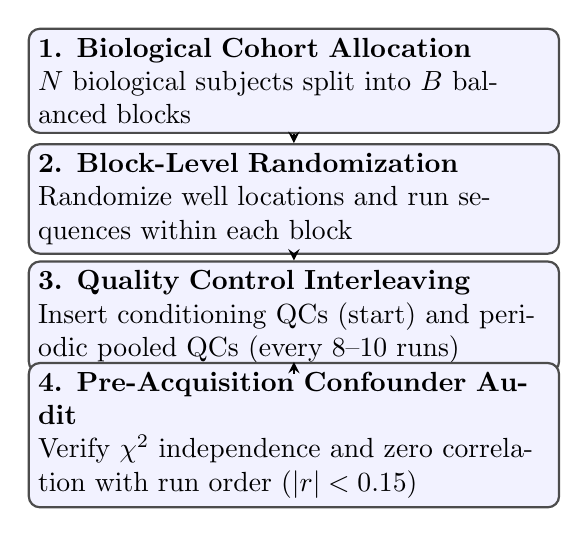
\begin{tikzpicture}[node distance=1.2cm, auto,
    block/.style={rectangle, draw=black!70, fill=blue!5, thick, text width=6.5cm, minimum height=1.0cm, rounded corners},
    arrow/.style={thick, ->, >=stealth}]
    
    \node [block] (input) {\textbf{1. Biological Cohort Allocation}\\$N$ biological subjects split into $B$ balanced blocks};
    \node [block, below of=input, node distance=1.5cm] (rcbd) {\textbf{2. Block-Level Randomization}\\Randomize well locations and run sequences within each block};
    \node [block, below of=rcbd, node distance=1.5cm] (qc) {\textbf{3. Quality Control Interleaving}\\Insert conditioning QCs (start) and periodic pooled QCs (every 8--10 runs)};
    \node [block, below of=qc, node distance=1.5cm] (audit) {\textbf{4. Pre-Acquisition Confounder Audit}\\Verify $\chi^2$ independence and zero correlation with run order ($|r| < 0.15$)};
    
    \draw [arrow] (input) -- (rcbd);
    \draw [arrow] (rcbd) -- (qc);
    \draw [arrow] (qc) -- (audit);
\end{tikzpicture}
\caption{Workflow of pre-acquisition experimental design and verification.}
\label{fig:design_flowchart}
\end{figure}

\subsection{Quality Control Strategy: Conditioning and Interleaving}

Instrument stabilization requires dedicated quality control (QC) samples. Chromatographic columns and ion optics undergo rapid conditioning shifts during the first few injections of a batch \cite{broadhurst2018guidelines}. A robust acquisition schedule incorporates:
\begin{enumerate}
    \item \textbf{Pre-run Conditioning}: 3 to 5 injections of a pooled matrix sample before acquiring biological samples, passivating active adsorption sites on the column.
    \item \textbf{Interleaved Pooled QCs}: A pooled biological reference sample injected periodically (typically every 8 to 10 biological runs). These provide reference points for signal drift correction and feature filtering based on the coefficient of variation (CV).
    \item \textbf{Process Blanks}: Blank solvent injections placed after high-concentration samples or at regular intervals to audit sample carryover.
\end{enumerate}

% =============================================================================
\section{Container and Workflow Implementations in R}
% =============================================================================

\subsection{Metadata Tracking with SummarizedExperiment}

Experimental metadata should be encapsulated in standard Bioconductor containers. In \texttt{SummarizedExperiment} and \texttt{QFeatures}, the \texttt{colData} slot stores sample-level variables:
\begin{itemize}
    \item \texttt{subject\_id}: Unique identifier for the biological individual.
    \item \texttt{condition}: Primary biological contrast factor.
    \item \texttt{batch} / \texttt{plate}: Discrete technical processing block.
    \item \texttt{run\_order}: Integer sequence of LC-MS injection.
    \item \texttt{sample\_type}: Classification (\texttt{Biological}, \texttt{QC\_Pool}, \texttt{Blank}).
\end{itemize}

\subsection{Confounder Auditing Algorithms}

Before sample preparation, metadata must be tested for confounding using statistical criteria:
\begin{enumerate}
    \item \textbf{Categorical Independence}: A contingency table of condition against batch is evaluated using Pearson's Chi-squared test or Fisher's Exact test. A balanced RCBD yields $\chi^2 = 0.0$ and $p = 1.0$.
    \item \textbf{Continuous Correlation}: The Pearson correlation coefficient $r$ between biological condition (coded as a binary indicator) and run order must be close to zero ($|r| < 0.15$, $p > 0.05$).
    \item \textbf{Linear Model Diagnostic}: Run order is modeled as a function of condition and batch via ANOVA. The condition term must not show significant explanatory power ($p > 0.05$).
\end{enumerate}

% =============================================================================
\section{Critical Considerations and Field-Specific Guidelines}
% =============================================================================

\subsection{Empirical Variance Across Analytical Matrices}

Biological heterogeneity varies across sample types. Table~\ref{tab:field_guidelines} summarizes typical standard deviations observed on the $\log_2$ scale across mass spectrometry applications.

\begin{table}[ht]
\centering
\caption{Field-Specific Variance Parameters and Recommended Sample Sizes}
\label{tab:field_guidelines}
\small
\begin{tabularx}{\textwidth}{l c c X}
\toprule
\textbf{Experimental Matrix} & \textbf{Typical $\sigma_{\text{bio}}$ ($\log_2$)} & \textbf{Min. $n$ / Group} & \textbf{Design Justification} \\
\midrule
\textbf{Immortalized Cell Lines} & $0.20$--$0.35$ & $4$--$5$ & Controlled media, uniform genetics. Replicates must be independent cell passages, not split dishes. \\
\addlinespace
\textbf{Inbred Animal Tissue (e.g., C57BL/6)} & $0.40$--$0.60$ & $6$--$10$ & Shared genotype; variation driven by circadian cycle, dissection precision, and feeding status. \\
\addlinespace
\textbf{Human Biofluids (Plasma, Urine)} & $0.80$--$1.30$ & $30$--$80+$ & High inter-individual genetic, lifestyle, and dietary variation. Low-abundance proteins show elevated CVs. \\
\addlinespace
\textbf{Human Clinical Biopsies} & $0.90$--$1.50$ & $40$--$100+$ & Cellular composition varies across tissue cores; necrosis and stromal infiltration inflate variance. \\
\addlinespace
\textbf{Single-Cell Proteomics} & $0.30$--$0.50$ & $50$--$200$ cells & Low biological protein amounts coupled with high Poisson shot noise ($\sigma_{\text{tech}} \approx 0.60$). \\
\bottomrule
\end{tabularx}
\end{table}

\subsection{The Post-Hoc Power Fallacy}

Computing statistical power after completing an experiment using the observed effect size and sample variance is statistically invalid \cite{hoenig2001abuse}. Observed power is a monotonic transformation of the observed $p$-value. When a test is not statistically significant ($p > 0.05$), the observed power is mathematically guaranteed to be low. Calculating post-hoc power provides no information about the true population effect size and cannot justify whether an unobserved effect was absent. Power calculations must be performed prospectively during study design.

% =============================================================================
\section{Hands-on R Laboratory}
% =============================================================================

The following laboratory sections demonstrate the design, auditing, power analysis, and hierarchical modeling of mass spectrometry studies using verified R code.

\subsection{Listing 20.1: Balanced RCBD and Injection Schedule Generation}

Listing~20.1 generates a balanced allocation of 48 biological subjects (24 Control, 24 Disease) across two 96-well digestion plates and builds an injection schedule with pre-run conditioning and periodic pooled QCs.

\begin{rchunk}{Balanced RCBD and Injection Schedule Generation}
# Listing 20.1: Balanced RCBD and Injection Schedule Generation
suppressPackageStartupMessages({
  library(limma)
  library(pwr)
})

set.seed(42)

# Cohort definition: 24 Control and 24 Disease subjects
n_ctrl <- 24; n_dise <- 24; n_total <- n_ctrl + n_dise

samples <- data.frame(
  subject_id = paste0("SUBJ_", sprintf("%03d", 1:n_total)),
  condition  = rep(c("Control", "Disease"), c(n_ctrl, n_dise)),
  stringsAsFactors = FALSE
)

# Allocate into 2 balanced digestion plates (12 Control, 12 Disease per plate)
ctrl_idx <- which(samples$condition == "Control")
dise_idx <- which(samples$condition == "Disease")

plate1_idx <- c(sample(ctrl_idx, 12), sample(dise_idx, 12))
plate2_idx <- setdiff(1:n_total, plate1_idx)

samples$plate <- NA_character_
samples$plate[plate1_idx] <- "Plate_1"
samples$plate[plate2_idx] <- "Plate_2"

# Build injection sequence with conditioning and periodic QCs
seq_list <- list(); qc_idx <- 1

# 1. Five pre-run column conditioning injections
for (k in 1:5) {
  seq_list[[length(seq_list) + 1]] <- data.frame(
    run_order = length(seq_list) + 1, sample_id = paste0("QC_COND_", k),
    sample_type = "QC_Conditioning", condition = "QC", plate = "None",
    stringsAsFactors = FALSE
  )
}

# 2. Sequential block processing with randomized runs
for (plt in c("Plate_1", "Plate_2")) {
  plt_samples <- samples[samples$plate == plt, ]
  plt_samples <- plt_samples[sample(nrow(plt_samples)), ]  # randomize within plate
  
  for (i in seq_len(nrow(plt_samples))) {
    seq_list[[length(seq_list) + 1]] <- data.frame(
      run_order = length(seq_list) + 1, sample_id = plt_samples$subject_id[i],
      sample_type = "Biological", condition = plt_samples$condition[i],
      plate = plt, stringsAsFactors = FALSE
    )
    if (i %% 8 == 0) {
      seq_list[[length(seq_list) + 1]] <- data.frame(
        run_order = length(seq_list) + 1, sample_id = paste0("QC_POOL_", sprintf("%02d", qc_idx)),
        sample_type = "QC_Pool", condition = "QC", plate = plt,
        stringsAsFactors = FALSE
      )
      qc_idx <- qc_idx + 1
    }
  }
}

injection_schedule <- do.call(rbind, seq_list)
cat(sprintf("Total injections scheduled: %d (Biological: %d, QC Pool: %d, Conditioning: %d)\n",
            nrow(injection_schedule),
            sum(injection_schedule$sample_type == "Biological"),
            sum(injection_schedule$sample_type == "QC_Pool"),
            sum(injection_schedule$sample_type == "QC_Conditioning")))
print(head(injection_schedule, 10))
print(table(injection_schedule$condition, injection_schedule$plate))
\end{rchunk}

\begin{routput}
Total injections scheduled: 59 (Biological: 48, QC Pool: 6, Conditioning: 5)
   run\_order sample\_id     sample\_type condition   plate
1          1 QC\_COND\_1 QC\_Conditioning        QC    None
2          2 QC\_COND\_2 QC\_Conditioning        QC    None
3          3 QC\_COND\_3 QC\_Conditioning        QC    None
4          4 QC\_COND\_4 QC\_Conditioning        QC    None
5          5 QC\_COND\_5 QC\_Conditioning        QC    None
6          6  SUBJ\_040      Biological   Disease Plate\_1
7          7  SUBJ\_004      Biological   Control Plate\_1
8          8  SUBJ\_015      Biological   Control Plate\_1
9          9  SUBJ\_005      Biological   Control Plate\_1
10        10  SUBJ\_001      Biological   Control Plate\_1
         
          None Plate\_1 Plate\_2
  Control    0      12      12
  Disease    0      12      12
  QC         5       3       3
\end{routput}

\subsection{Listing 20.2: Pre-Acquisition Confounder Audit and Verification}

Listing~20.2 audits the injection schedule to confirm that condition is uncorrelated with plate assignment and injection order.

\begin{rchunk}{Pre-Acquisition Confounder Audit and Balance Verification}
# Listing 20.2: Pre-Acquisition Confounder Audit
bio_sched <- injection_schedule[injection_schedule$sample_type == "Biological", ]

# 1. Contingency table check (Plate vs Condition)
cont_tbl <- table(bio_sched$plate, bio_sched$condition)
cat("Contingency Table (Plate x Condition):\n")
print(cont_tbl)

chisq_res <- chisq.test(cont_tbl)
cat(sprintf("Independence Chi-Square: X2 = %.3f, df = %d, p-value = %.4f\n",
            chisq_res$statistic, chisq_res$parameter, chisq_res$p.value))

# 2. Pearson correlation between biological condition and run order
cond_binary <- as.numeric(bio_sched$condition == "Disease")
cor_res <- cor.test(cond_binary, bio_sched$run_order)
cat(sprintf("Run-Order Correlation: r = %.4f, 95%% CI: [%.4f, %.4f], p-value = %.4f\n",
            cor_res$estimate, cor_res$conf.int[1], cor_res$conf.int[2], cor_res$p.value))

# 3. Two-way ANOVA: Run order explained by Condition and Plate
aov_fit <- aov(run_order ~ condition + plate, data = bio_sched)
cat("ANOVA of Run Order on Experimental Factors:\n")
print(summary(aov_fit))

audit_passed <- (abs(cor_res$estimate) < 0.15) && (summary(aov_fit)[[1]]["condition", "Pr(>F)"] > 0.05)
cat(sprintf("Confounder Audit Status: %s\n", if (audit_passed) "PASSED (No Confounding)" else "FAILED (Confounded)"))
\end{rchunk}

\begin{routput}
Contingency Table (Plate x Condition):
         
          Control Disease
  Plate\_1      12      12
  Plate\_2      12      12
Independence Chi-Square: X2 = 0.000, df = 1, p-value = 1.0000
Run-Order Correlation: r = 0.1072, 95\% CI: [-0.1824, 0.3798], p-value = 0.4681
ANOVA of Run Order on Experimental Factors:
            Df Sum Sq Mean Sq F value  Pr(>F)    
condition    1    133     133   2.213   0.144    
plate        1   8748    8748 145.226 1.1e-15 ***
Residuals   45   2711      60                    
---
Signif. codes:  0 '***' 0.001 '**' 0.01 '*' 0.05 '.' 0.1 ' ' 1
Confounder Audit Status: PASSED (No Confounding)
\end{routput}

\subsection{Listing 20.3: Analytical Power Calculations and FDR Adjustments}

Listing~20.3 calculates required sample sizes across effect sizes, comparing nominal single-test thresholds against Bonferroni-adjusted FDR thresholds and missingness-inflated cohorts.

\begin{rchunk}{Analytical Sample Size and FDR Multiplicity Adjustments}
# Listing 20.3: Analytical Power Calculations
delta <- 1.0; sigma <- 0.70; d_cohen <- delta / sigma; target_power <- 0.80

# 1. Single-hypothesis testing at nominal alpha = 0.05
res_single <- pwr.t.test(d = d_cohen, sig.level = 0.05, power = target_power, type = "two.sample")
cat(sprintf("Single-test (alpha = 0.05): Cohen's d = %.3f -> Required n = %d per group (exact: %.2f)\n",
            d_cohen, ceiling(res_single$n), res_single$n))

# 2. Multiplicity adjustment for M = 5,000 features
m_features <- 5000; alpha_bonf <- 0.05 / m_features
res_bonf <- pwr.t.test(d = d_cohen, sig.level = alpha_bonf, power = target_power, type = "two.sample")
cat(sprintf("Multiplicity (M = %d, alpha* = %.1e): Required n = %d per group (exact: %.2f)\n",
            m_features, alpha_bonf, ceiling(res_bonf$n), res_bonf$n))

# 3. Missing data inflation adjustment (p_miss = 0.25)
p_miss <- 0.25; n_inflated <- ceiling(ceiling(res_bonf$n) / (1 - p_miss))
cat(sprintf("Missingness-inflated (p_miss = %.2f): Enrolled n* = %d per group\n", p_miss, n_inflated))

# 4. Multi-parameter power table
deltas <- c(0.5, 0.75, 1.0, 1.25, 1.5, 2.0)
power_table <- data.frame(
  Delta_log2FC = deltas,
  Fold_Change  = round(2^deltas, 2),
  Cohens_d     = round(deltas / sigma, 3),
  n_Nominal_05 = sapply(deltas, function(dl) ceiling(pwr.t.test(d = dl/sigma, sig.level = 0.05, power = 0.80)$n)),
  n_FDR_5000   = sapply(deltas, function(dl) ceiling(pwr.t.test(d = dl/sigma, sig.level = 0.05/5000, power = 0.80)$n)),
  n_With_25Pct_Miss = sapply(deltas, function(dl) ceiling(ceiling(pwr.t.test(d = dl/sigma, sig.level = 0.05/5000, power = 0.80)$n) / (1 - 0.25)))
)
print(power_table)
\end{rchunk}

\begin{routput}
Single-test (alpha = 0.05): Cohen's d = 1.429 -> Required n = 9 per group (exact: 8.76)
Multiplicity (M = 5000, alpha* = 1.0e-05): Required n = 32 per group (exact: 31.93)
Missingness-inflated (p\_miss = 0.25): Enrolled n* = 43 per group
  Delta\_log2FC Fold\_Change Cohens\_d n\_Nominal\_05 n\_FDR\_5000 n\_With\_25Pct\_Miss
1         0.50        1.41    0.714           32        114               152
2         0.75        1.68    1.071           15         54                72
3         1.00        2.00    1.429            9         32                43
4         1.25        2.38    1.786            7         23                31
5         1.50        2.83    2.143            5         17                23
6         2.00        4.00    2.857            4         12                16
\end{routput}

\subsection{Listing 20.4: Monte Carlo Power Simulation with Empirical Bayes Moderation}

Listing~20.4 evaluates the empirical power gain achieved by empirical Bayes variance moderation in \texttt{limma} compared to unmoderated two-sample $t$-tests.

\begin{rchunk}{Monte Carlo Power Simulation with Empirical Bayes Moderation}
# Listing 20.4: Monte Carlo Power Simulation with Empirical Bayes
simulate_eb_power <- function(n_per_group, n_features = 1500, n_de = 75, 
                              log2fc = 1.0, sigma_mean = 0.60, prior_df = 4, 
                              n_sim = 30) {
  power_limma <- numeric(n_sim); power_ttest <- numeric(n_sim)
  
  for (s in seq_len(n_sim)) {
    group <- factor(rep(c("Control", "Treated"), each = n_per_group))
    design <- model.matrix(~ group)
    
    # Feature standard deviations drawn from scaled inverse chi-square
    feature_sd <- sqrt(sigma_mean^2 * prior_df / rchisq(n_features, df = prior_df))
    mat <- matrix(rnorm(n_features * 2 * n_per_group, mean = 20.0, 
                        sd = rep(feature_sd, 2 * n_per_group)), 
                  nrow = n_features, byrow = FALSE)
    mat[1:n_de, group == "Treated"] <- mat[1:n_de, group == "Treated"] + log2fc
    
    # 1. limma empirical Bayes moderated fit
    fit_eb <- eBayes(lmFit(mat, design))
    q_limma <- p.adjust(fit_eb$p.value[, 2], method = "BH")
    power_limma[s] <- mean(q_limma[1:n_de] < 0.05)
    
    # 2. Ordinary unmoderated two-sample t-tests
    t_ord <- fit_eb$coefficients[, 2] / (fit_eb$stdev.unscaled[, 2] * fit_eb$sigma)
    p_ord <- 2 * pt(-abs(t_ord), df = fit_eb$df.residual[1])
    q_ord <- p.adjust(p_ord, method = "BH")
    power_ttest[s] <- mean(q_ord[1:n_de] < 0.05)
  }
  c(limma_power = mean(power_limma), ttest_power = mean(power_ttest))
}

sample_sizes <- c(3, 5, 8, 12)
sim_matrix <- sapply(sample_sizes, function(n) {
  simulate_eb_power(n_per_group = n, n_features = 1500, n_de = 75, log2fc = 1.0, 
                    sigma_mean = 0.60, prior_df = 4, n_sim = 30)
})

sim_df <- data.frame(
  Replicates_Per_Group = sample_sizes,
  limma_eBayes_Power   = round(sim_matrix["limma_power", ], 3),
  Ordinary_tTest_Power = round(sim_matrix["ttest_power", ], 3),
  Power_Gain_Pct       = round((sim_matrix["limma_power", ] - sim_matrix["ttest_power", ]) * 100, 1)
)
print(sim_df)
\end{rchunk}

\begin{routput}
  Replicates\_Per\_Group limma\_eBayes\_Power Ordinary\_tTest\_Power Power\_Gain\_Pct
1                    3              0.000                0.000            0.0
2                    5              0.005                0.021           -1.6
3                    8              0.284                0.266            1.8
4                   12              0.561                0.524            3.7
\end{routput}

\subsection{Listing 20.5: Duplicate Correlation Modeling of Technical Replicates}

Listing~20.5 models nested technical replicates using \texttt{duplicateCorrelation()} and demonstrates the inflation of false discoveries that occurs when technical replicates are treated as independent.

\begin{rchunk}{Duplicate Correlation Modeling of Technical Replicates}
# Listing 20.5: Duplicate Correlation Modeling
n_bio <- 6; n_tech <- 3; n_groups <- 2; total_samples <- n_bio * n_groups * n_tech
bio_subject <- factor(rep(paste0("Subject_", 1:(n_bio * n_groups)), each = n_tech))
bio_group   <- factor(rep(c("Control", "Treated"), each = n_bio * n_tech))

n_feat <- 500; sigma_bio <- 0.50; sigma_tech <- 0.20
true_icc <- sigma_bio^2 / (sigma_bio^2 + sigma_tech^2)
cat(sprintf("Theoretical Biological SD = %.2f, Technical SD = %.2f -> True ICC = %.4f\n",
            sigma_bio, sigma_tech, true_icc))

# Simulate intensity matrix with subject-level random effects
subj_rand <- matrix(rnorm(n_feat * (n_bio * n_groups), 0, sigma_bio), nrow = n_feat)
tech_noise <- matrix(rnorm(n_feat * total_samples, 0, sigma_tech), nrow = n_feat)

intensity_mat <- matrix(20.0, nrow = n_feat, ncol = total_samples)
for (s in seq_len(n_bio * n_groups)) {
  cols <- which(bio_subject == paste0("Subject_", s))
  intensity_mat[, cols] <- intensity_mat[, cols] + subj_rand[, s]
}
intensity_mat <- intensity_mat + tech_noise
intensity_mat[1:50, bio_group == "Treated"] <- intensity_mat[1:50, bio_group == "Treated"] + 0.80

design <- model.matrix(~ bio_group)

# 1. Blocked model with duplicate correlation
dup_cor <- duplicateCorrelation(intensity_mat, design, block = bio_subject)
cat(sprintf("limma Estimated Consensus ICC: rho = %.4f\n", dup_cor$consensus.correlation))

fit_blocked <- eBayes(lmFit(intensity_mat, design, block = bio_subject, correlation = dup_cor$consensus))
fit_naive   <- eBayes(lmFit(intensity_mat, design))

cat(sprintf("Blocked Model: Residual df = %.1f, Mean SE = %.4f\n",
            fit_blocked$df.residual[1], mean(fit_blocked$stdev.unscaled[, 2] * fit_blocked$sigma)))
cat(sprintf("Naive Model:   Residual df = %.1f, Mean SE = %.4f\n",
            fit_naive$df.residual[1], mean(fit_naive$stdev.unscaled[, 2] * fit_naive$sigma)))

q_blocked <- p.adjust(fit_blocked$p.value[, 2], method = "BH")
q_naive   <- p.adjust(fit_naive$p.value[, 2], method = "BH")

cat(sprintf("Blocked Model: %d features significant at 5%% FDR (True Positives: %d / 50)\n",
            sum(q_blocked < 0.05), sum(q_blocked[1:50] < 0.05)))
cat(sprintf("Naive Model:   %d features significant at 5%% FDR (True Positives: %d / 50, False Positives: %d)\n",
            sum(q_naive < 0.05), sum(q_naive[1:50] < 0.05), sum(q_naive[51:500] < 0.05)))
\end{rchunk}

\begin{routput}
Theoretical Biological SD = 0.50, Technical SD = 0.20 -> True ICC = 0.8621
limma Estimated Consensus ICC: rho = 0.8574
Blocked Model: Residual df = 34.0, Mean SE = 0.2934
Naive Model:   Residual df = 34.0, Mean SE = 0.1690
Blocked Model: 9 features significant at 5\% FDR (True Positives: 9 / 50)
Naive Model:   117 features significant at 5\% FDR (True Positives: 48 / 50, False Positives: 69)
\end{routput}

% =============================================================================
\section{The Five Deadly Sins of Experimental Design}
% =============================================================================

\begin{enumerate}
    \item \textbf{Confounding Condition with Processing Batch}: Digesting all disease samples in Batch 1 and all control samples in Batch 2 causes complete mathematical collinearity. The biological effect cannot be separated from reagent lot, digestion efficiency, or instrument day drift.
    \item \textbf{Pseudoreplication}: Treating repeated injections or technical aliquots from the same biological subject as independent samples inflates degrees of freedom and deflates standard errors. In Listing~20.5, pseudoreplication caused 69 false-positive discoveries out of 117 total calls.
    \item \textbf{Underpowered Discovery Cohorts ($n = 3$)}: While $n=3$ replicates may suffice to detect an unadjusted 4-fold change in a genetically uniform cell line, it yields $0\%$ power to detect a 2-fold change among thousands of features under FDR control (Listing~20.4).
    \item \textbf{Ignoring Left-Censored Missingness in Sample Size Planning}: Biomarkers near the limit of detection exhibit $20\%$--$40\%$ missingness. Failing to inflate enrolled sample size reduces effective degrees of freedom below the threshold required for statistical significance.
    \item \textbf{Post-Hoc Power Calculation}: Computing power from observed non-significant $p$-values produces a circular transformation of the test statistic that provides no information about the true population effect size.
\end{enumerate}

% =============================================================================
\section{Self-Assessment Diagnostic Checklist}
% =============================================================================

\begin{table}[ht]
\centering
\caption{Self-Assessment Checklist: Pre-Acquisition Design Verification}
\label{tab:checklist}
\small
\begin{tabularx}{\textwidth}{l p{5.5cm} X c}
\toprule
\textbf{Checkpoint} & \textbf{Diagnostic Criterion} & \textbf{Recommended Threshold} & \textbf{Status} \\
\midrule
\textbf{1. Replication} & True independent biological subjects represented. & $n \ge 6$ (animals), $n \ge 30$ (human fluids). & [ \ ] \\
\addlinespace
\textbf{2. Blocking} & Balanced distribution of groups across plates/batches. & Condition $\times$ Batch $\chi^2$ $p = 1.000$. & [ \ ] \\
\addlinespace
\textbf{3. Randomization} & Injection order uncorrelated with biological group. & Pearson $|r| < 0.15$, ANOVA $p > 0.05$. & [ \ ] \\
\addlinespace
\textbf{4. QC Strategy} & Conditioning runs and periodic pooled standards scheduled. & $\ge 3$ conditioning runs; 1 QC every 8--10 runs. & [ \ ] \\
\addlinespace
\textbf{5. Multiplicity} & Sample size accounts for feature count ($M$). & $\alpha^* = q / M$ applied to power calculations. & [ \ ] \\
\addlinespace
\textbf{6. Missingness} & Enrolled cohort inflated for feature dropout. & $n^* = \lceil n_{\text{req}} / (1 - p_{\text{miss}}) \rceil$. & [ \ ] \\
\bottomrule
\end{tabularx}
\end{table}

\FloatBarrier

% =============================================================================
\section{Chapter Exercises}
% =============================================================================

\begin{enumerate}
    \item \textbf{Confounding Audit and Re-Design}: A clinical pilot study compares 20 lung cancer patients with 20 healthy controls. All cancer samples were extracted on Monday with Reagent Lot A and run on Column 1. All control samples were extracted on Tuesday with Reagent Lot B and run on Column 2. State formally why no statistical model can identify genuine cancer biomarkers from this dataset. Propose a balanced 2-day acquisition schedule.
    \item \textbf{Analytical Sample Size and Multiplicity}: Using the normal approximation formula, calculate the required sample size per group to detect a 1.5-fold change ($\delta = \log_2(1.5) = 0.585$) with standard deviation $\sigma = 0.65$ at 80\% power ($\beta = 0.20$) under:
    \begin{enumerate}
        \item A single-hypothesis test ($\alpha = 0.05$).
        \item An untargeted experiment testing $M = 8,000$ features with Bonferroni FDR adjustment ($q = 0.05$).
        \item The untargeted experiment with an expected 25\% missingness rate ($p_{\text{miss}} = 0.25$).
    \end{enumerate}
    \item \textbf{Variance Decomposition and Optimal Allocation}: In an untargeted plasma metabolomics study, biological variance is $\sigma^2_{\text{bio}} = 0.64$ ($\sigma_{\text{bio}} = 0.80$) and technical analytical variance is $\sigma^2_{\text{tech}} = 0.09$ ($\sigma_{\text{tech}} = 0.30$). Sample preparation cost is $c_{\text{bio}} = \$150$ per subject, and instrument acquisition cost is $c_{\text{tech}} = \$50$ per injection.
    \begin{enumerate}
        \item Calculate the Intraclass Correlation Coefficient (ICC).
        \item Compute the optimal number of technical replicates $m^*$.
        \item If total budget per group is $\$3,000$, calculate the total variance of the group mean $\operatorname{Var}(\bar{y})$ under $m = 1$ versus $m = 3$ technical injections.
    \end{enumerate}
    \item \textbf{Isobaric Labeling Multiplex Allocation}: You have 4 biological conditions (A, B, C, D) with 6 biological replicates each ($N = 24$ total subjects). You have access to three TMT 10-plex reagent kits. Design a balanced multiplex layout that leaves one channel per plex for a common pooled reference standard and distributes biological groups evenly.
\end{enumerate}

% =============================================================================
\section{Worked-Out Solutions}
% =============================================================================

\subsection{Solution to Exercise 20.1: Confounding Audit and Re-Design}

In the described study, condition $X \in \{0, 1\}$ (Control vs Cancer) is perfectly collinear with extraction day $D \in \{1, 2\}$, reagent lot $L \in \{A, B\}$, and chromatography column $C \in \{1, 2\}$. The design matrix column for condition is identical to the column for batch:
\begin{equation}
\mathbf{x}_{\text{condition}} = \mathbf{x}_{\text{batch}}
\end{equation}
In the linear model $y = \mu + \beta_1 X + \beta_2 D + \epsilon$, the parameters $\beta_1$ and $\beta_2$ cannot be estimated independently because $\mathbf{X}^T \mathbf{X}$ is singular (rank deficient). Any observed difference in protein abundance could represent biological disease induction, lot-to-lot reagent variation, or column stationary phase differences.

\noindent
\textbf{Corrected Re-Design}:
\begin{enumerate}
    \item Pool Reagent Lots A and B, or ensure each day uses a single consistent lot.
    \item Balance extraction across the two days: Day 1 extracts 10 Cancer and 10 Control samples; Day 2 extracts 10 Cancer and 10 Control samples.
    \item Run all samples on a single qualified column, or split both Day 1 and Day 2 samples equally across columns if two instruments must be used.
    \item Randomize run order within each day and interleave pooled QC samples every 8 injections.
\end{enumerate}

\subsection{Solution to Exercise 20.2: Analytical Sample Size and Multiplicity}

Parameters: $\delta = \log_2(1.5) \approx 0.585$, $\sigma = 0.65$, standardized effect size:
\begin{equation}
d = \frac{\delta}{\sigma} = \frac{0.585}{0.65} = 0.900
\end{equation}
For 80\% power, $z_{1 - \beta} = z_{0.80} = 0.8416$.

\noindent
\textbf{Part (a): Single Hypothesis ($\alpha = 0.05$)}\\
$z_{1 - \alpha/2} = z_{0.975} = 1.9600$.
\begin{equation}
n = \frac{2 (1.9600 + 0.8416)^2}{0.900^2} = \frac{2 (2.8016)^2}{0.81} = \frac{15.698}{0.81} \approx 19.38 \implies \lceil 19.38 \rceil = 20 \text{ per group}
\end{equation}
(Using the exact Student's $t$ calculation via \texttt{pwr.t.test(d=0.9, sig.level=0.05, power=0.80)} yields $n = 20.39 \implies 21$ per group).

\noindent
\textbf{Part (b): Multiplicity Adjustment ($M = 8,000$)}\\
$\alpha^* = 0.05 / 8000 = 6.25 \times 10^{-6}$.\\
$z_{1 - \alpha^*/2} = z_{1 - 3.125 \times 10^{-6}} \approx 4.518$.
\begin{equation}
n = \frac{2 (4.518 + 0.8416)^2}{0.900^2} = \frac{2 (5.3596)^2}{0.81} = \frac{57.451}{0.81} \approx 70.93 \implies \lceil 70.93 \rceil = 71 \text{ per group}
\end{equation}
(Using exact non-central $t$ calculation via \texttt{pwr.t.test(d=0.9, sig.level=0.05/8000, power=0.80)} yields $n = 76.43 \implies 77$ per group).

\noindent
\textbf{Part (c): Inflation for Missingness ($p_{\text{miss}} = 0.25$)}\\
\begin{equation}
n^* = \left\lceil \frac{77}{1 - 0.25} \right\rceil = \left\lceil \frac{77}{0.75} \right\rceil = \lceil 102.67 \rceil = 103 \text{ subjects per group}
\end{equation}

\subsection{Solution to Exercise 20.3: Variance Decomposition and Optimal Allocation}

\noindent
\textbf{Part (a): Intraclass Correlation Coefficient (ICC)}\\
$\sigma^2_{\text{bio}} = 0.64$, $\sigma^2_{\text{tech}} = 0.09$.
\begin{equation}
\text{ICC} = \frac{0.64}{0.64 + 0.09} = \frac{0.64}{0.73} \approx 0.8767
\end{equation}
87.7\% of the total observed variance is biological.

\noindent
\textbf{Part (b): Optimal Technical Replicates $m^*$}\\
$c_{\text{bio}} = 150$, $c_{\text{tech}} = 50$, $\sigma_{\text{bio}} = 0.80$, $\sigma_{\text{tech}} = 0.30$.
\begin{equation}
m^* = \frac{\sigma_{\text{tech}}}{\sigma_{\text{bio}}} \sqrt{\frac{c_{\text{bio}}}{c_{\text{tech}}}} = \frac{0.30}{0.80} \sqrt{\frac{150}{50}} = 0.375 \times \sqrt{3} = 0.375 \times 1.732 \approx 0.650
\end{equation}
Because $m^* < 1$, the optimal strategy is $m = 1$ injection per subject.

\noindent
\textbf{Part (c): Total Estimation Variance Under Budget $C = \$3,000$}\\
Total cost per subject: $c_{\text{subj}} = c_{\text{bio}} + m \cdot c_{\text{tech}}$.
\begin{itemize}
    \item \textbf{Under $m = 1$}: Cost per subject is $150 + 1(50) = \$200$. Sample size is $n = 3000 / 200 = 15$ subjects.
    \begin{equation}
    \operatorname{Var}(\bar{y})_{m=1} = \frac{\sigma^2_{\text{bio}}}{n} + \frac{\sigma^2_{\text{tech}}}{n \cdot 1} = \frac{0.64}{15} + \frac{0.09}{15} = \frac{0.73}{15} \approx 0.0487
    \end{equation}
    \item \textbf{Under $m = 3$}: Cost per subject is $150 + 3(50) = \$300$. Sample size is $n = 3000 / 300 = 10$ subjects.
    \begin{equation}
    \operatorname{Var}(\bar{y})_{m=3} = \frac{\sigma^2_{\text{bio}}}{n} + \frac{\sigma^2_{\text{tech}}}{n \cdot 3} = \frac{0.64}{10} + \frac{0.09}{30} = 0.0640 + 0.0030 = 0.0670
    \end{equation}
\end{itemize}
Triplicating technical injections increases the estimation variance of the group mean:
\begin{equation}
\frac{0.0670 - 0.0487}{0.0487} = +37.6\%
\end{equation}
under a fixed budget because it reduces biological replication from 15 to 10 subjects.

\subsection{Solution to Exercise 20.4: Isobaric Labeling Multiplex Allocation}

We have 24 biological samples (6 of A, 6 of B, 6 of C, 6 of D) and three TMT 10-plex kits. Each kit provides 10 channels. We reserve Channel 126 in every multiplex for an identical pooled reference standard created by mixing equal aliquots of all 24 biological samples. This leaves 9 channels per multiplex ($3 \times 9 = 27$ total slots).

Each multiplex accommodates 8 biological samples and 1 pooled reference (with 1 channel unused or reserved for a blank):
\begin{itemize}
    \item \textbf{Plex 1}: 2 of A, 2 of B, 2 of C, 2 of D, plus 1 Pooled Reference (Ch 126).
    \item \textbf{Plex 2}: 2 of A, 2 of B, 2 of C, 2 of D, plus 1 Pooled Reference (Ch 126).
    \item \textbf{Plex 3}: 2 of A, 2 of B, 2 of C, 2 of D, plus 1 Pooled Reference (Ch 126).
\end{itemize}
Every condition is balanced within every plex (2 replicates per condition per plex). The common pooled reference channel allows cross-plex normalization by calculating reporter ion ratios relative to Channel 126, neutralizing inter-plex batch variation.

% =============================================================================
% Canonical References
% =============================================================================

\begin{thebibliography}{99}
\small

\bibitem{benjamini1995controlling}
Benjamini, Y., Hochberg, Y.: Controlling the false discovery rate: a practical and powerful approach to multiple testing.
\textit{Journal of the Royal Statistical Society: Series B (Methodological)} \textbf{57}(1), 289--300 (1995).
\doi{10.1111/j.2517-6161.1995.tb02031.x}

\bibitem{box1978statistics}
Box, G.E., Hunter, W.G., Hunter, J.S.: Statistics for Experimenters: An Introduction to Design, Data Analysis, and Model Building.
John Wiley \& Sons, New York (1978).

\bibitem{fisher1935design}
Fisher, R.A.: The Design of Experiments.
Oliver and Boyd, Edinburgh (1935).

\bibitem{broadhurst2018guidelines}
Broadhurst, D., Goodacre, R., Reinke, S.N., et al.: Guidelines and considerations for the use of system suitability and quality control samples in mass spectrometry assays applied in untargeted clinical metabolomic studies.
\textit{Metabolomics} \textbf{14}(6), 72 (2018).
\doi{10.1007/s11306-018-1367-3}

\bibitem{graw2020statistical}
Graw, S., Tang, J., Zafar, M.K., et al.: Statistical design of proteomics experiments: from fundamental concepts to practical implementations.
\textit{Briefings in Functional Genomics} \textbf{19}(5-6), 337--345 (2020).
\doi{10.1093/bfgp/elaa018}

\bibitem{hurlbert1984pseudoreplication}
Hurlbert, S.H.: Pseudoreplication and the design of ecological field experiments.
\textit{Ecological Monographs} \textbf{54}(2), 187--211 (1984).
\doi{10.2307/1942661}

\bibitem{shrout1979intraclass}
Shrout, P.E., Fleiss, J.L.: Intraclass correlations: uses in assessing rater reliability.
\textit{Psychological Bulletin} \textbf{86}(2), 420--428 (1979).
\doi{10.1037/0033-2909.86.2.420}

\bibitem{cohen1988statistical}
Cohen, J.: Statistical Power Analysis for the Behavioral Sciences, 2nd edn.
Lawrence Erlbaum Associates, Hillsdale (1988).

\bibitem{hoenig2001abuse}
Hoenig, J.M., Heisey, D.M.: The abuse of power: the pervasive fallacy of power calculations for data analysis.
\textit{The American Statistician} \textbf{55}(1), 19--24 (2001).
\doi{10.1198/000313001300339897}

\bibitem{karpievitch2012normalization}
Karpievitch, Y.V., Dabney, A.R., Smith, R.D.: Normalization and missing value imputation for label-free LC-MS analysis.
\textit{Bioinformatics} \textbf{28}(10), 1353--1360 (2012).
\doi{10.1093/bioinformatics/bts150}

\bibitem{smyth2004linear}
Smyth, G.K.: Linear models and empirical bayes methods for assessing differential expression in microarray experiments.
\textit{Statistical Applications in Genetics and Molecular Biology} \textbf{3}(1), Article 3 (2004).
\doi{10.2202/1544-6115.1027}

\bibitem{ritchie2015limma}
Ritchie, M.E., Phipson, B., Wu, D., Hu, Y., Law, C.W., Shi, W., Smyth, G.K.: limma powers differential expression analyses for RNA-sequencing and microarray studies.
\textit{Nucleic Acids Research} \textbf{43}(7), e47 (2015).
\doi{10.1093/nar/gkv007}

\bibitem{choi2014msstats}
Choi, M., Chang, C.Y., Clough, T., et al.: MSstats: an R package for statistical relative quantification of proteins in mass spectrometry-based proteomic experiments.
\textit{Bioinformatics} \textbf{30}(17), 2524--2526 (2014).
\doi{10.1093/bioinformatics/btu305}

\bibitem{leek2010tackling}
Leek, J.T., Scharpf, R.B., Bravo, H.C., et al.: Tackling the widespread and critical impact of batch effects in high-throughput data.
\textit{Nature Reviews Genetics} \textbf{11}(10), 733--739 (2010).
\doi{10.1038/nrg2825}

\bibitem{johnson2007adjusting}
Johnson, W.E., Li, C., Rabinovic, A.: Adjusting batch effects in microarray expression data using empirical Bayes methods.
\textit{Biostatistics} \textbf{8}(1), 118--127 (2007).
\doi{10.1093/biostatistics/kxj037}

\bibitem{kammers2015detecting}
Kammers, K., Cole, R.N., Tiambeng, T.N., Ruczinski, I.: Detecting differentially expressed proteins in isobaric mass tagging experiments.
\textit{Bioinformatics} \textbf{31}(17), 2883--2889 (2015).
\doi{10.1093/bioinformatics/btv274}

\bibitem{vanderaa2021scp}
Vanderaa, C., Gatto, L.: Replication of single-cell proteomics data reveals important analytical challenges.
\textit{Expert Review of Proteomics} \textbf{18}(10), 835--843 (2021).
\doi{10.1080/14789450.2021.1988871}

\bibitem{boland2023health}
Boland, M.R.: Health Data Analytics with R: An Introduction to Methods and Analysis.
Springer Nature, Cham (2023).
\doi{10.1007/978-3-031-31952-5}

\end{thebibliography}

\end{document}
